\documentclass[12pt]{article}
\usepackage[spanish]{babel}
\usepackage[utf8]{inputenc}

% Extras
\usepackage{url}
\usepackage{hyperref}
\usepackage{float}  % H

% Código
\usepackage{courier}
\usepackage{listings}
\lstset{basicstyle=\footnotesize\ttfamily,breaklines=true}

% Imágenes
\usepackage{graphicx}
\usepackage{subcaption}
\graphicspath{{images/}}

% Cambio de la fuente de las secciones
\usepackage{setspace}
\usepackage{sectsty}
\allsectionsfont{\normalfont\scshape}

% Configuración página
\usepackage{vmargin}
\setmarginsrb{3 cm}{2.5 cm}{3 cm}{2.5 cm}{1 cm}{1.5 cm}{1 cm}{1.5 cm}
\usepackage{fancyhdr}
\pagestyle{fancy}
%\lhead{\thetitle}
\cfoot{\thepage}

% Configuración portada
\title{Proyecto de Clasificación: Exploración de Datos}			% Título
\author{Daniel González Alonso\\		% Autor
        Joshua Miguel González Santana\\
		Javier Estefanía González}
\date{\today}							% Fecha

\makeatletter
\let\thetitle\@title
\let\theauthor\@author
\let\thedate\@date
\makeatother


%%%%%%%%%%%%%%%%%%%%%%%%%%%%%%%%%%%%%%%%%%%%%%%%%%%%%%%%%%%%%%%%%%%%%%%%%%%%%%%%%%%%%%%%%
\begin{document}

%%%%%%%%%% PORTADA %%%%%%%%%%
\begin{titlepage}
	\centering
    \vspace*{0.25 cm}
    %\includegraphics[scale = 0.75]{UVa_logo2.jpg}\\[1.0 cm]	% Logo Universidad
    %\textsc{\LARGE Universidad de Valladolid}\\[1.5 cm]			% Nombre Universidad
	%\textsc{\Large Escuela de Ingeniería Informática}\\[0.5 cm]	% Nombre Escuela
	%\textsc{\large Estadística Descriptiva}\\[0.5 cm]			% Nombre Curso
	
	\doublespacing
	\textsc{\LARGE Máster Universitario en Inteligencia de Negocio y Big Data en Entornos Seguros}\\[0.5 cm]
	\singlespacing
	\textsc{\large Técnicas de Aprendizaje Automático Escalables}\\[0.5 cm]
	
	\rule{\linewidth}{0.2 mm}\\[0.4 cm]
	\textsc{\huge \bf \thetitle}\\
	\rule{\linewidth}{0.2 mm}\\[2.5 cm]
	
	\begin{minipage}{0.6\textwidth}
		\begin{flushleft} \large
			\emph{Autores:}\\
			\begin{itemize}
            	\item[] \theauthor
            \end{itemize}
		\end{flushleft}
	\end{minipage}~
	\begin{minipage}{0.3\textwidth}
		\begin{flushright} \large
		\end{flushright}
	\end{minipage}\\[6 cm]
	{\large \thedate}\\[2 cm]

	\vfill	
\end{titlepage}

%%%%%%%%%% INDICE %%%%%%%%%%
\tableofcontents
\pagebreak

%%%%%%%%%%%%%%%%%%%%%%%%%%%%%%%%%%%%%%%%%%%%%%%%%%%%%%%%%%%%%%%%%%%%%%%%%%%%%%%%%%%%%%%%%
\section{Introducción}
Este documento es el primero de una serie de entregables que conforman una actividad de evaluación con el tema \textbf{Proyecto de clasificación} que consistirá, en último término y de acuerdo con el enunciado, en comparar el rendimiento de dos clasificadores de la biblioteca de Spark ML trabajando sobre dataframes, para un conjunto de datos seleccionado. Este primer entregable  está enfocado a la descripción y la exploración de los datos, sin modificar el conjunto original de datos.\\

En las diferentes secciones, se realiza una descripción del conjunto de datos incluyendo información sobre su origen, los archivos y registros que lo conforman, los tipos de información que almacenan y detalles particulares de los atributos que incluye. Después, se describe el problema que se desea resolver en particular dentro del alcance de este trabajo.\\

Más tarde se describen el conjunto de datos, atributo por atributo, incluyendo estadísticas y gráficas que ilustren la información contenida. Por último,  se examina la correlación entre los datos existentes y se extraen las conclusiones a esta primera etapa de análisis.

%%%% DESCRIPCIÓN %%%%
\section{Descripción del conjunto de datos}
El conjunto de datos seleccionado ha sido \textit{NYC Taxi Trip Duration}, un conjunto proporcionado por la plataforma \textit{Kaggle}. Este set forma parte de una competición organizada por dicha plataforma, con el objetivo de intentar predecir la duración total de los trayectos en taxi en la ciudad de Nueva York. Esta información, correspondiente al año 2016, proviene en última instancia de la \textit{Comisión de Taxis y Limusinas de Nueva York}. La fuente del conjunto de datos es la siguiente: \url{https://www.kaggle.com/c/nyc-taxi-trip-duration/data}.\\

El conjunto de interés de estos datos está formado por 2 archivos diferentes. En ambos casos, cada uno de los registros representa un trayecto o viaje realizado por un proveedor del servicio.
\begin{itemize}
    \item \texttt{train.csv}: Este archivo tiene un tamaño aproximado de 190 Mb y $1.5$ millones de registros y está orientado a ser usado como conjunto de datos de entrenamiento, puesto que uno de los atributos que contiene, son las duraciones de los trayectos.
    \item \texttt{test.csv}: Este archivo tiene un tamaño aproximado de 65 Mb y 600.000 registros. A diferencia del archivo de \textit{train}, este  fichero no contiene las duraciones de los trayectos.
\end{itemize}
Los diferentes atributos de los que constan los archivos son:
\begin{enumerate}
    \item \texttt{id}: Se trata de un identificador único para cada trayecto, como una cadena de texto.
    \item \texttt{vendor\_id}: Identificador del proveedor del servicio. Este identificador está formado por un número entero.
    \item \texttt{pickup\_datetime}: Fecha y hora a la que el taxímetro se conectó.
    \item \texttt{dropoff\_datetime}: Fecha y hora a la que el taxímetro se desconectó.
    \item \texttt{passenger\_count}: Número de pasajeros en el vehículo. Este campo toma valores enteros de naturaleza discreta.
    \item \texttt{pickup\_longitude}: Longitud geográfica en la que el taxímetro se conectó.
    \item \texttt{pickup\_latitude}: Latitud geográfica en la que el taxímetro se conectó.
    \item \texttt{dropoff\_longitude}: Longitud geográfica en la que el taxímetro se desconectó.
    \item \texttt{dropoff\_latitude}: Latitud geográfica en la que el taxímetro se desconectó.
    \item \texttt{store\_and\_fwd\_flag}: Esta marca indica si el registro de viaje se mantuvo en la memoria del vehículo antes de enviarlo al proveedor, porque el vehículo no tenía una conexión con el servidor. Los valores que puede tomar son: Y = Almacenado y enviado; N = Trayecto no almacenado y enviado. Por lo que estamos ante un atributo de naturaleza booleana.
    \item \texttt{trip\_duration}: Se trata de la duración del trayecto, expresada en segundos.
\end{enumerate}

\newpage
%%%% EXPLORACIÓN DE DATOS %%%%
\section{Exploración de datos}
\subsection{Descripción del problema}
El problema a resolver es la predicción de la duración total de los trayectos en la ciudad de Nueva York. Es decir, se busca obtener registros formados por un Id único del trayecto, seguido de la predicción de duración para ese trayecto (en segundos, al igual que en el fichero \texttt{train.csv} descrito anteriormente). La siguiente tabla sirve como ejemplo de los resultados deseados.

\begin{table}[H]
\centering
\begin{tabular}{|p{2.5cm}|p{2.5cm}|}
\hline
id & trip\_duration\\ \hline
id3004672      & 959  \\ \hline
id3004673      & 874  \\ \hline
\end{tabular}
\caption{Ejemplo de formato de la solución buscada al problema}
\end{table}

Al formar parte de una competición pública de Kaggle, ya existen multitud de soluciones a este mismo problema las cuales pueden ser consultadas en \url{https://www.kaggle.com/c/nyc-taxi-trip-duration/code}.\\


\subsection{Descripción del conjunto de datos}

La descripción del conjunto de datos (véase la propuesta en el tema 2.2, apartado 3) aporta información de interés para la limpieza y transformación de datos.


\begin{itemize}
    \item Atributo \texttt{passenger\_count}:
    
Es el número de pasajeros transportados por el taxi durante el trayecto. Se encuentra almacenado como números enteros. Las estadísticas básicas extraídas de este atributo se muestran a continuación:

\begin{table}[H]
\begin{tabular}{|p{2.5cm}|p{2.5cm}|p{2.5cm}|p{2.5cm}|p{2.5cm}|}
\hline
Cardinalidad & MIN         & MAX        & AVG        & STDEV    \\ \hline
1458644      & 0 & 9 & 1.664530 & 1.314242 \\ \hline
\end{tabular}
\caption{Estadísticas del atributo \texttt{dropoff\_longitude}}
\end{table}

Por otro lado, también se ha obtenido un gráfico de barras de este atributo con el fin de facilitar la visualización de la distribución de los datos:

\begin{figure}[H]
    \centering
    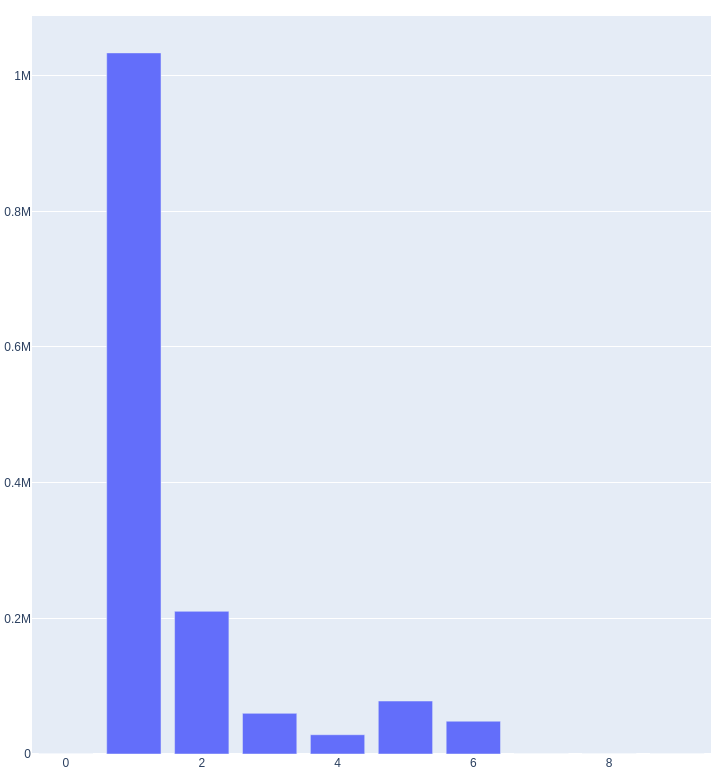
\includegraphics[width=0.75\textwidth]{passenger_count.PNG}
    \caption{Distribución del atributo \texttt{passenger\_count}}
    \label{fig:passenger_count}
\end{figure}

En la figura podemos apreciar que el valor más frecuente es, con diferencia, el número 1, lo cual nos indica que la mayor parte de los trayectos realizados por los proveedores de servicios se realizan para 1 solo pasajero, esto está alineado con el dato de la media calculado en las estadísticas del atributo.

%%%%%%%%%%%%%%%%%%%%%%%%%%%%%%%%%%%%%%%%%%%%%%%%%%%%%%%%%%%%%%%%%%%%%%%%%%%%%%%%%%%%%%%
\item Atributo \texttt{vendor\_id}:
    
Es el identificador del proveedor del servicio. Se encuentra almacenado como números enteros, que pueden tomar el valor   1 o 2.

\begin{table}[H]
\centering
\begin{tabular}{|c|c|c|}
\hline
Id         & Total     & Tanto por ciento  \\ \hline
\textit{1}  & 678342     & $46.5049\%$      \\ \hline
\textit{2}  & 780302   & $53.4950\%$      \\ \hline
\end{tabular}
\caption{Estadísticas del atributo \texttt{vendor\_id}}
\end{table}

Por otro lado, también se ha obtenido un gráfico de barras de este atributo con el fin de facilitar la visualización de la distribución de los datos:

\begin{figure}[H]
    \centering
    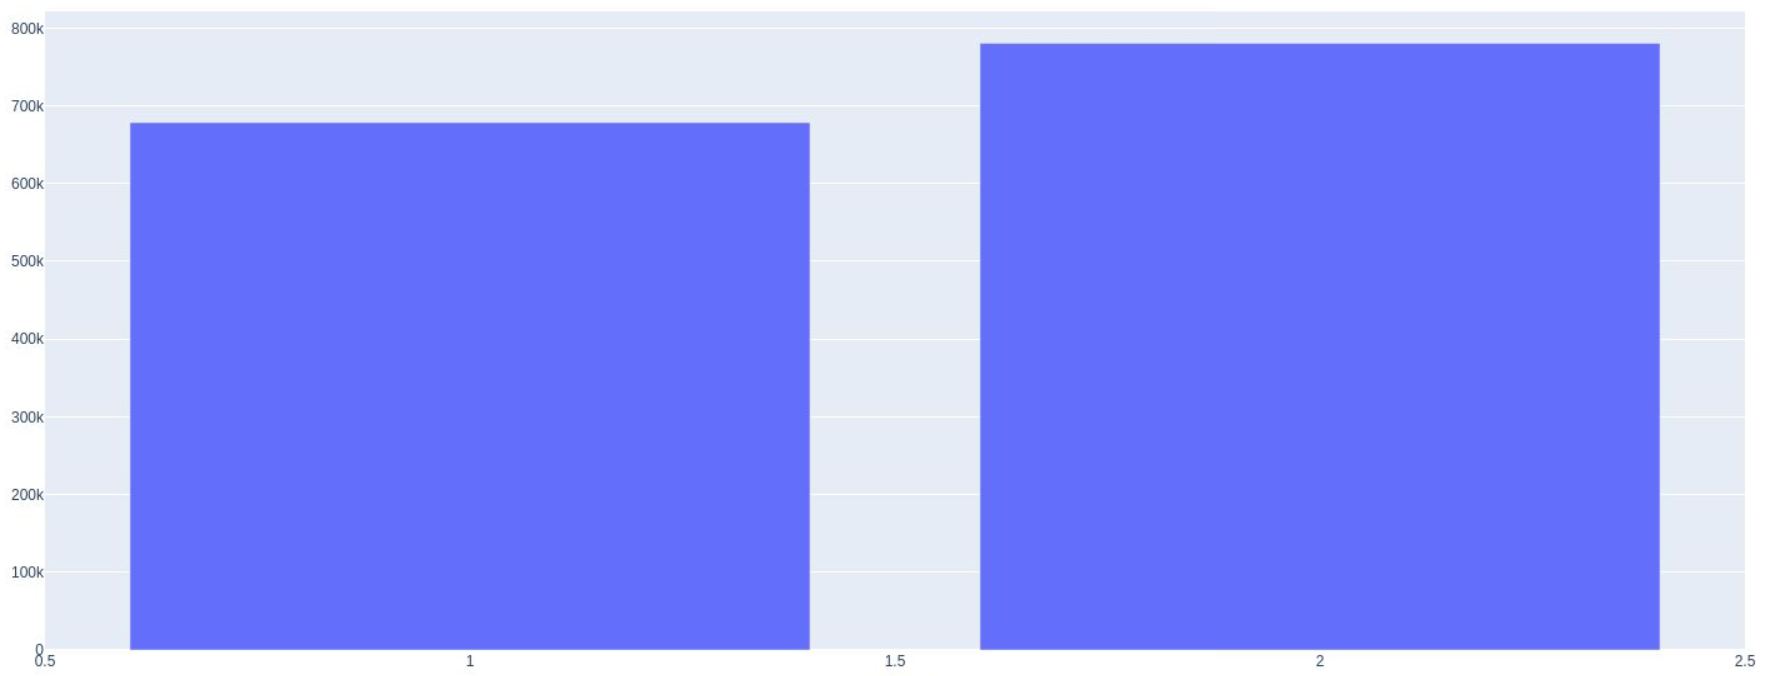
\includegraphics[width=0.75\textwidth]{vendor_id.PNG}
    \caption{Distribución del atributo \texttt{vendor\_id}}
    \label{fig:passenger_count}
\end{figure}

La figura ilustra que el proveedor de servicio $2$ ha sido el más utilizado en el periodo de tiempo en el que se recogieron los datos, con una diferencia de más de $10000$ registros.

    \item Atributo \texttt{dropoff\_longitude}:

Es la longitud geográfica donde se desconectó el taxímetro del taxi. Se encuentra almacenado como números decimales Double.

\begin{table}[H]
\centering
\begin{tabular}{|p{2.5cm}|p{2.5cm}|p{2.5cm}|p{2.5cm}|p{2.5cm}|}
\hline
Cardinalidad & MIN         & MAX        & AVG        & STDEV    \\ \hline
1458644      & -121.933304 & -61.335529 & -73.973416 & 0.070643 \\ \hline
\end{tabular}
\caption{Estadísticas del atributo \texttt{dropoff\_longitude}}
\end{table}

Por otro lado, también se ha obtenido un histograma de este atributo con el fin de facilitar la visualización de la dispersión de los datos:

\begin{figure}[H]
    \centering
    \begin{subfigure}{0.5\textwidth}
        \centering
        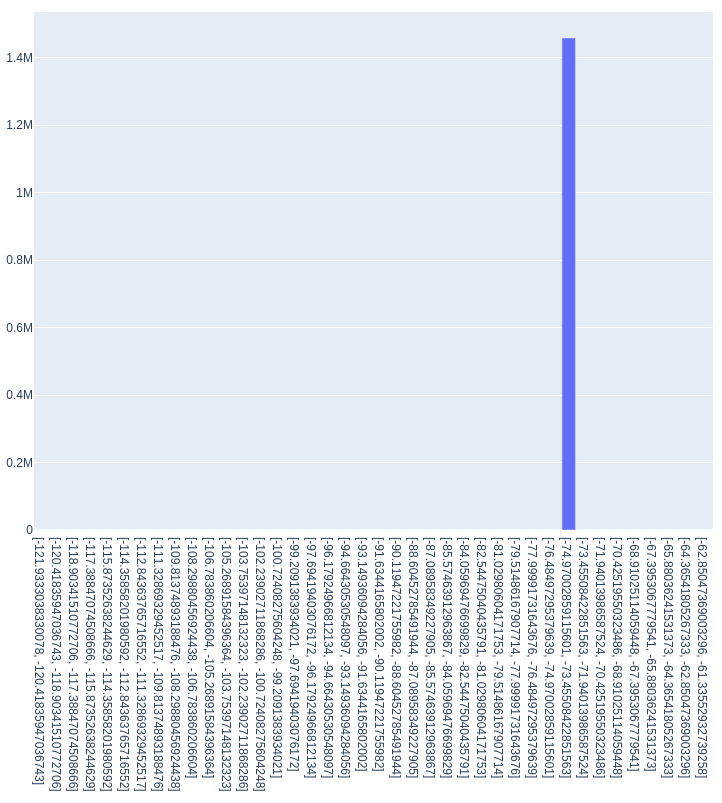
\includegraphics[width=1\textwidth]{dropoff_longitude.PNG}
        \label{fig:sub_dropoff_longitude}
        \caption{Gráfico completo}
    \end{subfigure}%
    \begin{subfigure}{0.5\textwidth}
        \centering
        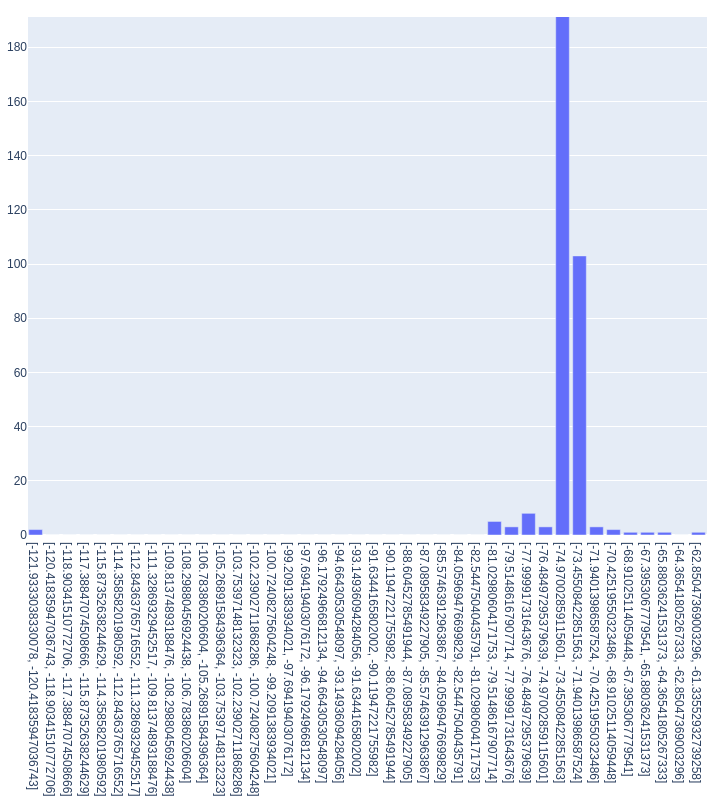
\includegraphics[width=1\textwidth]{dropoff_longitude_recortado.PNG}
        \label{fig:sub_dropoff_longitude_recortado}
        \caption{Gráfico recortado}
    \label{fig:sub2}
    \end{subfigure}
    \caption{Distribución del atributo \texttt{dropoff\_longitude}}
    \label{fig:dropoff_longitude}
\end{figure}

    \item Atributo \texttt{dropoff\_latitude}:

Es la latitud geográfica donde se desconectó el taxímetro del taxi. Se encuentra almacenado como un número decimal Double. Las estadísticas básicas extraídas de este atributos se muestran a continuación:

\begin{table}[H]
\centering
\begin{tabular}{|p{2.5cm}|p{2.5cm}|p{2.5cm}|p{2.5cm}|p{2.5cm}|}
\hline
Cardinalidad & MIN         & MAX        & AVG        & STDEV    \\ \hline
1458644      & 32.181141 & 43.921028 & 40.751800 & 0.035891 \\ \hline
\end{tabular}
\caption{Estadísticas del atributo \texttt{dropoff\_longitude}}
\end{table}

Por otro lado, también se ha obtenido un histograma de este atributo con el fin de facilitar la visualización de la dispersión de los datos:

\begin{figure}[H]
    \centering
    \begin{subfigure}{0.5\textwidth}
        \centering
        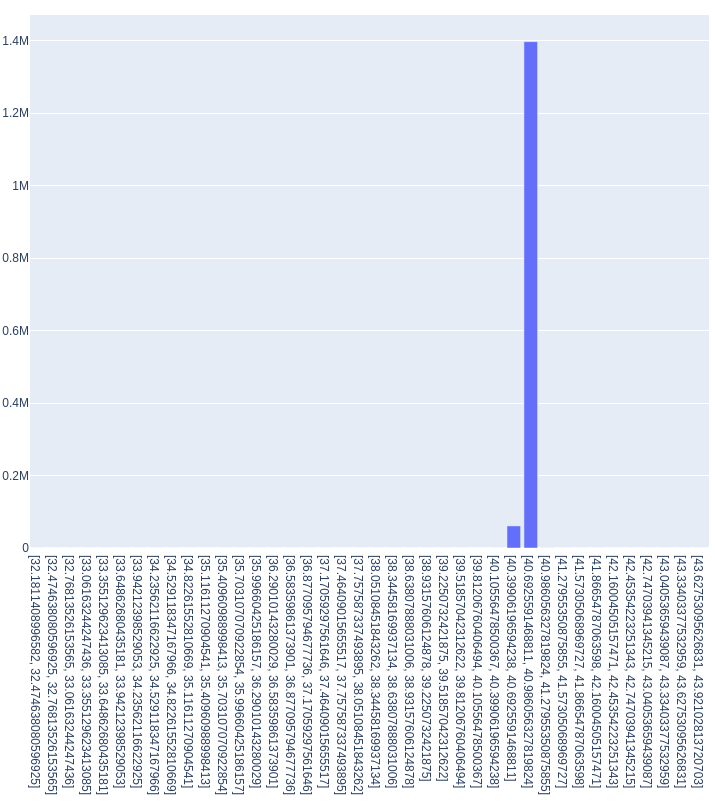
\includegraphics[width=1\textwidth]{dropoff_latitude.PNG}
        \label{fig:sub_dropoff_latitude}
        \caption{Gráfico completo}
    \end{subfigure}%
    \begin{subfigure}{0.5\textwidth}
        \centering
        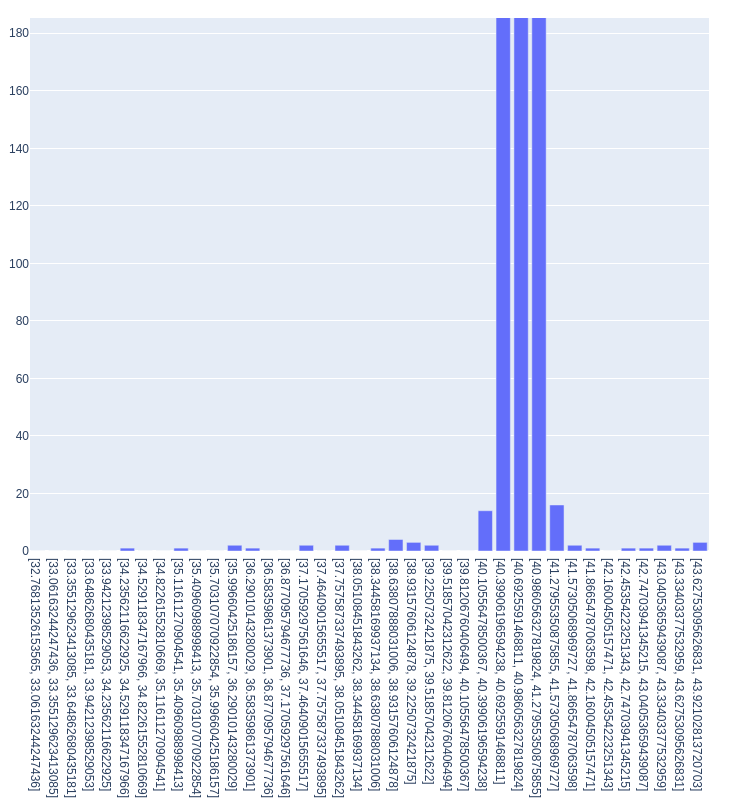
\includegraphics[width=1\textwidth]{dropoff_latitude_recortado.PNG}
        \label{fig:sub_dropoff_latitude_recortado}
        \caption{Gráfico recortado}
    \label{fig:sub2}
    \end{subfigure}
    \caption{Distribución del atributo \texttt{dropoff\_latitude}}
    \label{fig:dropoff_latitude}
\end{figure}

   \item Atributo \texttt{pickup\_latitude}:

Es la latitud geográfica donde se conectó el taxímetro del taxi. Se encuentra almacenado como un número decimal Double. Las estadísticas básicas extraídas de este atributos se muestran a continuación:

\begin{table}[H]
\centering
\begin{tabular}{|p{2.5cm}|p{2.5cm}|p{2.5cm}|p{2.5cm}|p{2.5cm}|}
\hline
Cardinalidad & MIN         & MAX        & AVG        & STDEV    \\ \hline
1458644      & 34.359695 & 51.881084 & 40.750921 & 0.032881 \\ \hline
\end{tabular}
\caption{Estadísticas del atributo \texttt{pickup\_latitude}}
\end{table}

Por otro lado, también se ha obtenido un histograma de este atributo con el fin de facilitar la visualización de la dispersión de los datos:

\begin{figure}[H]
    \centering
    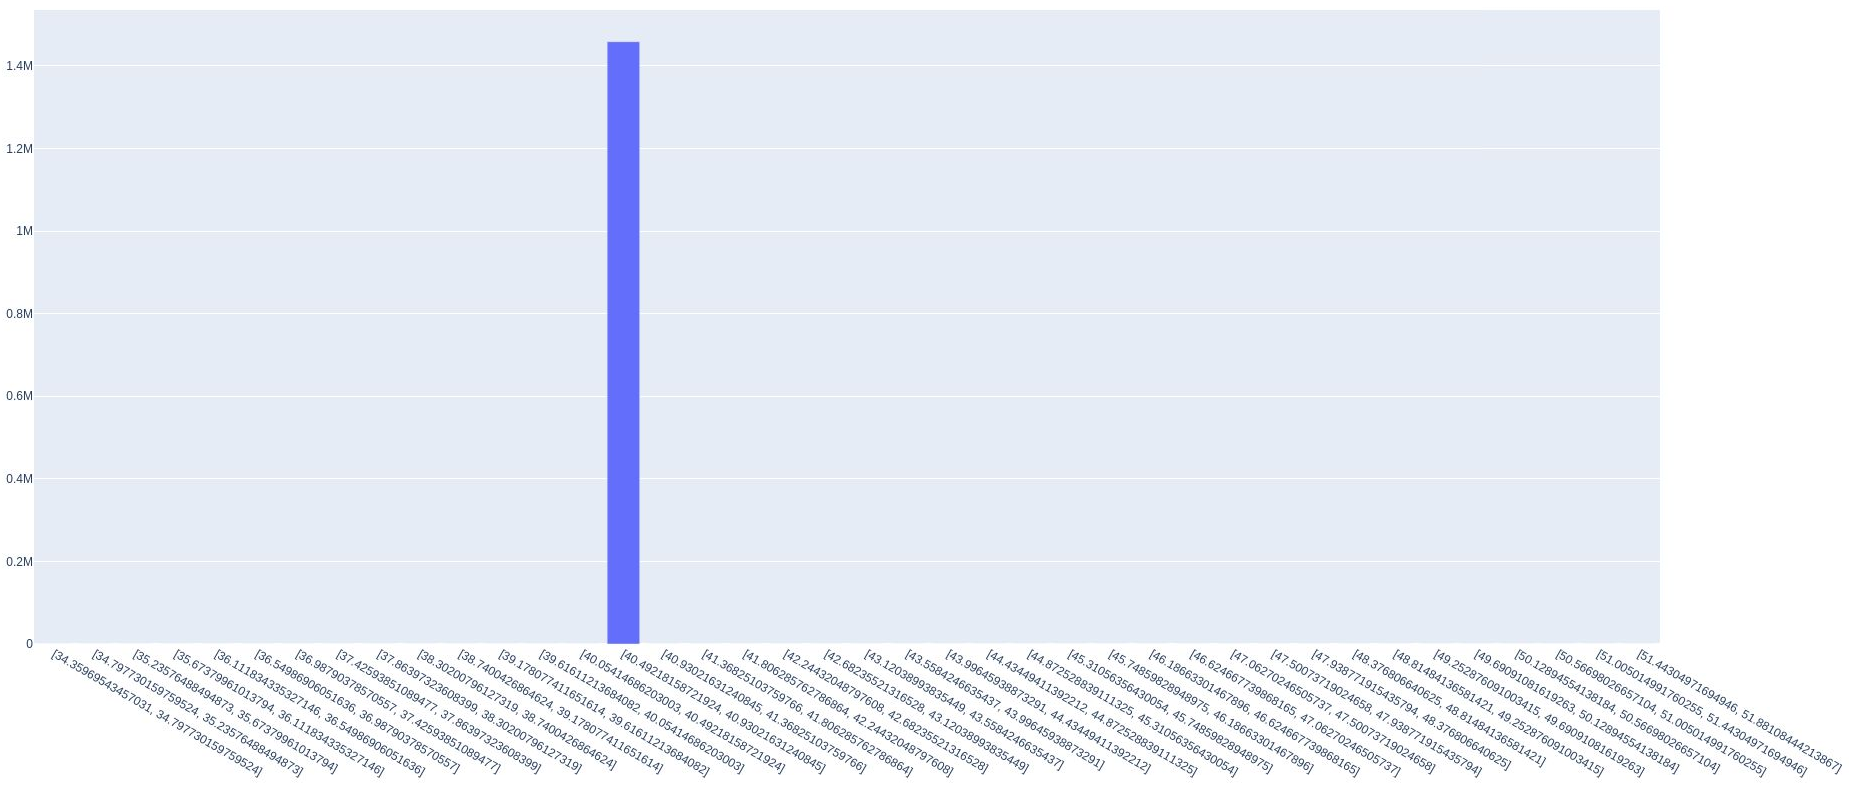
\includegraphics[width=0.75\textwidth]{pickup_latitude.png}
    \caption{Distribución del atributo \texttt{pickup\_latitude}}
    \label{fig:pickup_latitude}
\end{figure}
%%%%%%%%%%%%%%%%%%%%%%%%%%%%%%%%%%%%%%%%%%%%%%%%%%%%%%%%%%%%%%%%%%%%%%%%%%%%%%%%%%%%%%%%%%%%%%%%%%%%%%
\item Atributo \texttt{pickup\_longitude}:

Es la longitud geográfica donde se conectó el taxímetro del taxi. Se encuentra almacenado como un número decimal Double. Las estadísticas básicas extraídas de este atributos se muestran a continuación:

\begin{table}[H]
\centering
\begin{tabular}{|p{2.5cm}|p{2.5cm}|p{2.5cm}|p{2.5cm}|p{2.5cm}|}
\hline
Cardinalidad & MIN         & MAX        & AVG        & STDEV    \\ \hline
1458644      & -121.933342 & -61.335529 & -73.973486 & 0.070902 \\ \hline
\end{tabular}
\caption{Estadísticas del atributo \texttt{pickup\_longitude}}
\end{table}

Por otro lado, también se ha obtenido un histograma de este atributo con el fin de facilitar la visualización de la dispersión de los datos:

\begin{figure}[H]
    \centering
    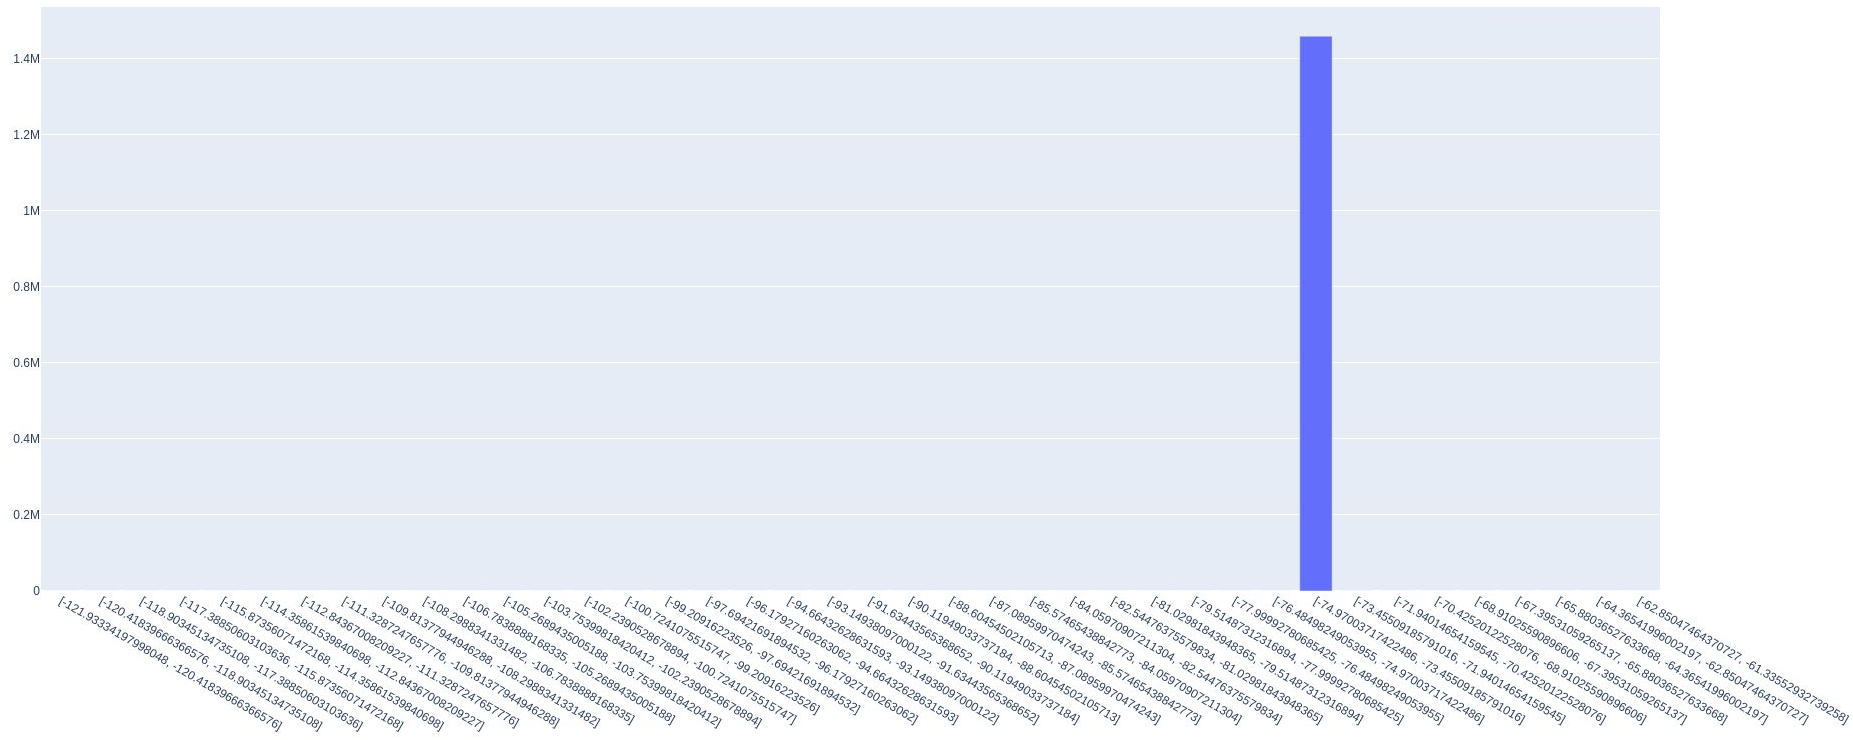
\includegraphics[width=0.75\textwidth]{pickup_longitude.png}
    \caption{Distribución del atributo \texttt{pickup\_longitude}}
    \label{fig:pickup_longitude}
\end{figure}
%%%%%%%%%%%%%%%%%%%%%%%%%%%%%%%%%%%%%%%%%%%%%%%%%%%%%%%%%%%%%%%%%%%%%%%%%%%%%%%%%%%%%%%%%%%%%%%%%%%%%%%%%%%%%%%
    \item Atributo \texttt{store\_and\_fwd\_flag}:

Es una bandera empleada para indicar si el registro del viaje se almacenó en la memoria del vehículo antes de enviarlo al proveedor, posiblemente porque el vehículo no tenía una conexión con el servidor. Se encuentra almacenado como un único carácter que puede tomar los siguientes valores:
    
    \begin{itemize}
        \item \textit{Y} = Almacenado y enviado.
        \item \textit{N} = Trayecto no almacenado y enviado.
    \end{itemize}

La distribución de este atributo es la siguiente:

\begin{table}[H]
\centering
\begin{tabular}{|c|c|c|}
\hline
Tag         & Total     & Tanto por ciento  \\ \hline
\textit{Y}  & 8045      & $0.551539\%$      \\ \hline
\textit{N}  & 1450599   & $99.44846\%$      \\ \hline
\end{tabular}
\caption{Estadísticas del atributo \texttt{dropoff\_longitude}}
\end{table}

    \item Atributo \texttt{pickup\_datetime}:

Es la fecha y la hora a la que el taxímetro se conectó. Este timestamp está almacenado como un String con formato \texttt{AAAA-MM-DD hh:mm:ss}.

La distribución de este atributo es la siguiente:

\begin{figure}[H]
    \centering
    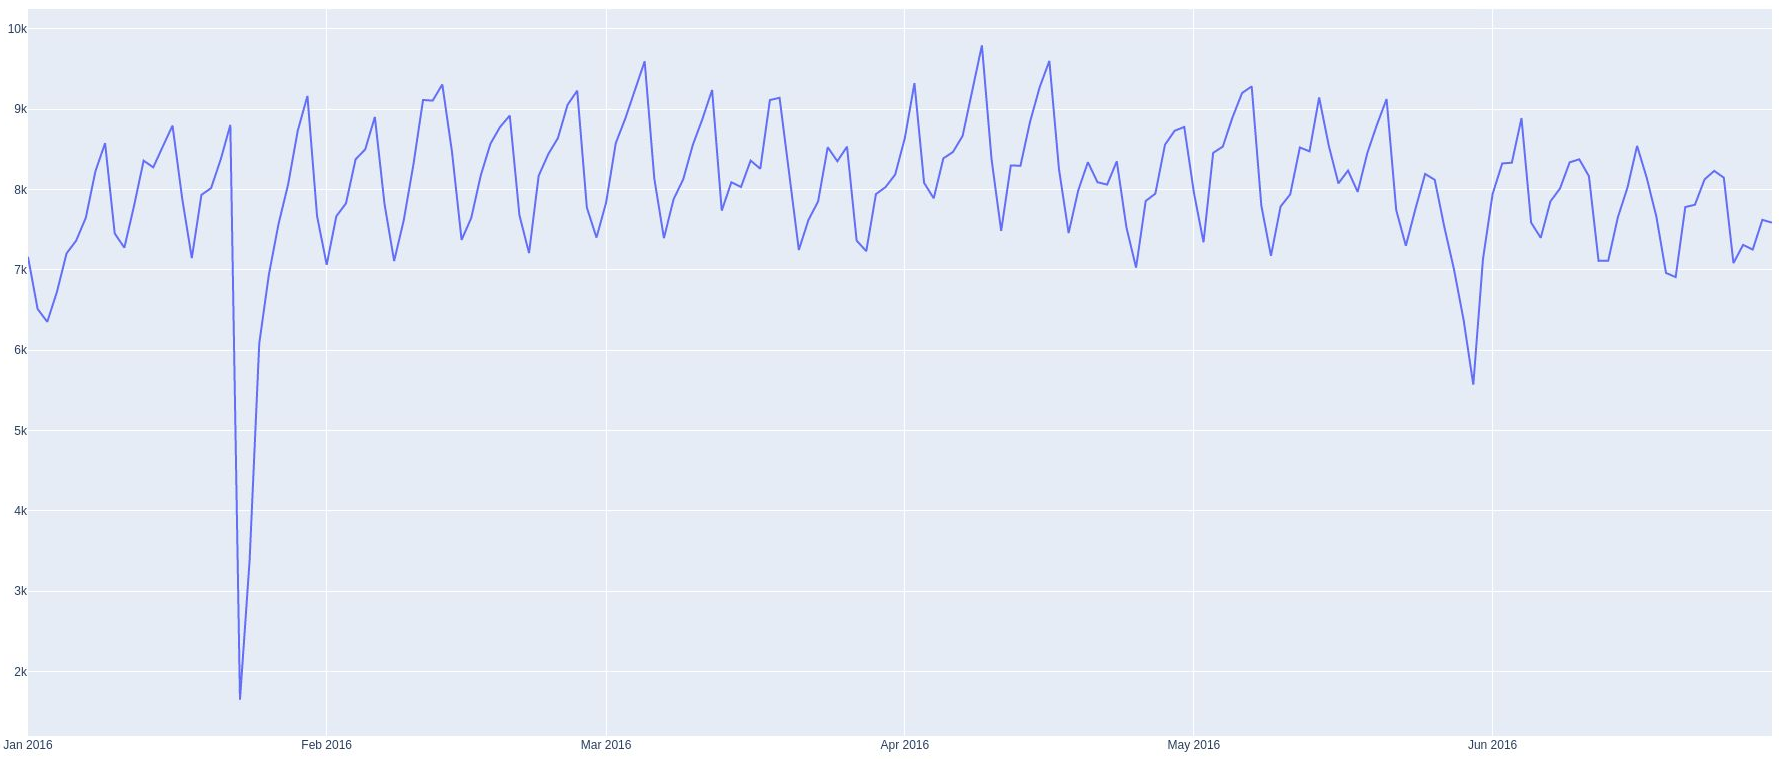
\includegraphics[width=0.8\textwidth]{pickup_datetime.PNG}
    \caption{Distribución del atributo \texttt{pickup\_datetime}}
    \label{fig:dropoff_datetime}
\end{figure}

En la figura, se puede ver que la serie temporal está comprendida entre Enero y Julio del año 2016. En el eje vertical, vemos que la mayor parte de los datos se encuentran contenidos en el rango entre 6K y 10K, a excepción de 2 fechas notables que permanecen por debajo de este rango, llegando al valor de 2k en su punto más extremo.\\

Una de estas fechas, el 23 de enero de 2016, posiblemente se debió a un importante temporal de nieve que causó el bloqueo total de la ciudad.

    \item Atributo \texttt{dropoff\_datetime}:

Es la fecha y la hora a la que el taxímetro se desconectó. Este timestamp está almacenado como un String con formato \texttt{AAAA-MM-DD hh:mm:ss}.

La distribución de este atributo es la siguiente:

\begin{figure}[H]
    \centering
    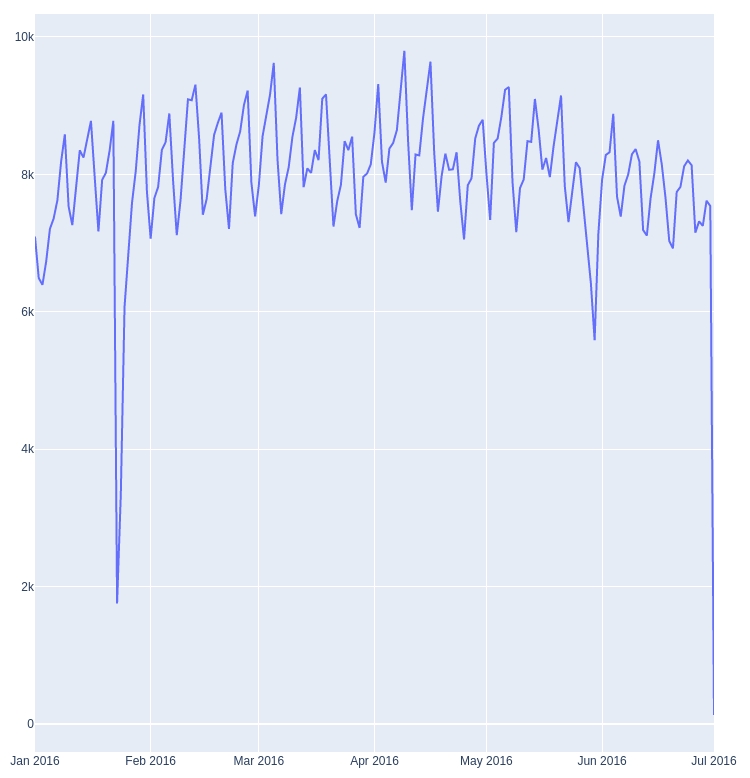
\includegraphics[width=0.8\textwidth]{dropoff_datetime.PNG}
    \caption{Distribución del atributo \texttt{dropoff\_datetime}}
    \label{fig:dropoff_datetime}
\end{figure}

Igual que podíamos apreciar en el atributo anterior, en esta figura podemos apreciar que la serie temporal está comprendida entre Enero  y Julio del año 2016. En el eje vertical, vemos que la mayor parte de los datos se encuentran contenidos en el rango entre 6K y 10K, a excepción de 2 fechas notables.

Como se puede observar, el 23 de enero de 2016 hay una caída importante en el número de viajes. Esto no es un error. Ese día Nueva York tuvo un importante temporal de nieve que causó el bloqueo total de la ciudad \cite{BBC}.
\end{itemize}
\newpage
\subsection{Examinar correlaciones en los datos}

Se ha decidido hacer una análisis de correlación para poder conocer si existen atributos redundantes que pudiesen ser descartados. En nuestro caso se ha decidido calcular la correlación entre todos los atributos descartando \texttt{id}, ya que el ser único no va a haber ninguna correlación, y los \texttt{pickup\_datetime} y \texttt{dropoff\_datetime}, ya que al ser \textit{timestamps} no se va obtener tampoco ninguna correlación. El resultado de estos cálculos se representa en el siguiente \textit{heatmap} de correlaciones:

\begin{figure}[H]
    \centering
    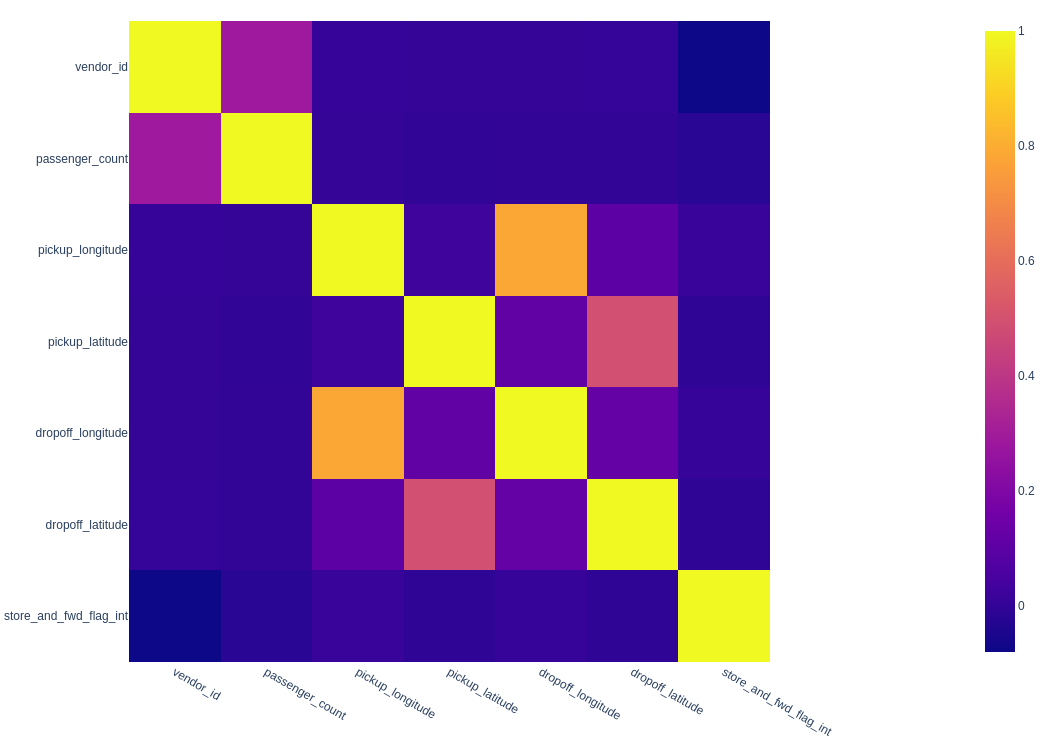
\includegraphics[width=1.0\textwidth]{correlaciones.PNG}
    \caption{Correlaciones entre diversos atributos}
    \label{fig:correlaciones}
\end{figure}

Como se puede ver la correlación entre atributos es escasa, las mayores las encontramos entre los atributos \texttt{pickup\_latitude} y \texttt{dropoff\_latitude} con $0.494037$, y entre \texttt{pickup\_longitude} y \texttt{dropoff\_longitude} con $0.783581$, lo cual tiene sentido ya que habrá muchas personas que repetirán recorridos de una forma habitual, como por ejemplo, para ir al trabajo.\\

Teniendo en cuenta que no se tienen muchos atributos y que estas correlaciones no son muy elevadas, no se debería descartar ningún atributo.

\newpage


%%%%%%%%%%%%%%% CONCLUSIONES %%%%%%%%%%%%%%
\section{Conclusiones}
En esta sección se recogen las diferentes conclusiones obtenidas tras el análisis realizado al conjunto de datos a tratar. A saber:
\begin{itemize}
    \item El conjunto de datos original está compuesto de 2 archivos y un total de $2.1$ millones de registros.
    \item Se han analizado los 11 atributos diferentes que conforman el archivo \texttt{train.csv} mediante estadísticas y de forma visual. Pero ha de tenerse en cuenta que uno de los requisitos de esta entrega era la no modificación del set de datos origina.
    \item El problema a resolver trata de predecir la duración en segundos de diferentes trayectos.
    \item Cada trayecto con identificador único debe ser tomado como válido y sin repetición, ya que varios vehículos podrían estar realizando el mismo trayecto al mismo tiempo, o el mismo trayecto podría estar siendo realizado por diferentes proveedores de servicio. No se han encontrado valores vacíos. 
    \item Existen fechas puntales en las que el volumen de registros fue notablemente más bajo, identificados mediante gráficos de los atributos. A estos datos se les ha buscado un contexto histórico para verificar su veracidad.\cite{BBC}. Además, los viajes registrados en el último día del conjunto de datos, corresponderían a aquellos que finalizaron en dicho día, es decir, cuyo \texttt{dropoff\_datetime} es de ese último día y cuyo \texttt{dropoff\_datetime} comenzó en el día anterior.
    \item Tras el examen de correlación entre los atributos, no se debería eliminar ninguno de ellos por tener índices de correlación bajos. Las mayores correlaciones existentes son entre los atributos \texttt{pickup\_latitude} y \texttt{dropoff\_latitude}, así como  entre \texttt{pickup\_longitude} y \texttt{dropoff\_longitude}
    
\end{itemize}
\newpage

\section{Esfuerzo}

La distribución del esfuerzo realizado en el análisis, compresión, redacción y coordinación de este documento ha sido la siguiente:

\begin{table}[H]
\centering
\begin{tabular}{|c|c|c|}
\hline
Alumno         & Esfuerzo (Hr)    & Tanto por ciento  \\ \hline
\textit{Daniel Gonzalez Alonso}  &   12    & $33.3\%$      \\ \hline
\textit{Joshua M. González Santana}  & 5   & $33.3\%$      \\ \hline
\textit{Javier Estefanía González}  & 12  & $33.3\%$      \\ \hline
\end{tabular}
\caption{Carga de trabajo de los alumnos}
\end{table}

%%%%%%%%%% REFERENCIAS
\section{Bibliografía}
\begin{thebibliography}{0}
	\bibitem{kaggle}
      Kaggle,
      \emph{New York City Taxi Trip Duration},
      \url{https://www.kaggle.com/c/nyc-taxi-trip-duration/code}
    \bibitem{BBC}
      BBC,
      \emph{La gigantesca tormenta de nieve que clausuró a Nueva York},
      \url{https://www.bbc.com/mundo/noticias/2016/01/160123_eeuu_nueva_york_tormenta_emergencia_ab}
\end{thebibliography}

\end{document}
